\documentclass[12pt]{article}

%%%%%%%%%%%%%%%%%%%%%%%%%%%%%%%%%%%%%%%%%%%%%%%%%%%%%%%%%%%%%%%%%%%%%%%%%%%%%%%%
%                           Package preset for homework
%%%%%%%%%%%%%%%%%%%%%%%%%%%%%%%%%%%%%%%%%%%%%%%%%%%%%%%%%%%%%%%%%%%%%%%%%%%%%%%%
% Miscellaneous
\usepackage[margin=1in]{geometry}
\usepackage[utf8]{inputenc}
\usepackage{indentfirst}
\usepackage{blindtext}
\usepackage{graphicx}
\usepackage{xr-hyper}
\usepackage{hyperref}
\usepackage{enumitem}
\usepackage{color}
\usepackage{float}
% Math
\usepackage{latexsym}
\usepackage{amsfonts}
\usepackage{amssymb}
\usepackage{amsmath}
\usepackage{commath}
\usepackage{amsthm}
\usepackage{bbold}
\usepackage{bm}
% Physics
\usepackage{physics}
\usepackage{siunitx}
% Code typesetting
\usepackage{listings}
% Citation
\usepackage[authoryear]{natbib}
\usepackage{appendix}
\usepackage[capitalize]{cleveref}
% Title & name
\title{Homework}
\author{Tien Vo}
\date{\today}


%%%%%%%%%%%%%%%%%%%%%%%%%%%%%%%%%%%%%%%%%%%%%%%%%%%%%%%%%%%%%%%%%%%%%%%%%%%%%%%%
%                   User-defined commands and environments
%%%%%%%%%%%%%%%%%%%%%%%%%%%%%%%%%%%%%%%%%%%%%%%%%%%%%%%%%%%%%%%%%%%%%%%%%%%%%%%%
%%% Misc
\sisetup{load-configurations=abbreviations}
\newcommand{\due}[1]{\date{Due: #1}}
\newcommand{\hint}{\textit{Hint}}
\let\oldt\t
\renewcommand{\t}[1]{\text{#1}}

%%% Bold sets & abbrv
\newcommand{\N}{\mathbb{N}}
\newcommand{\Z}{\mathbb{Z}}
\newcommand{\R}{\mathbb{R}}
\newcommand{\Q}{\mathbb{Q}}
\let\oldP\P
\renewcommand{\P}{\mathbb{P}}
\newcommand{\LL}{\mathcal{L}}
\newcommand{\FF}{\mathcal{F}}
\newcommand{\HH}{\mathcal{H}}
\newcommand{\NN}{\mathcal{N}}
\newcommand{\ZZ}{\mathcal{Z}}
\newcommand{\RN}[1]{\textup{\uppercase\expandafter{\romannumeral#1}}}
\newcommand{\ua}{\uparrow}
\newcommand{\da}{\downarrow}

%%% Unit vectors
\newcommand{\xhat}{\vb{\hat{x}}}
\newcommand{\yhat}{\vb{\hat{y}}}
\newcommand{\zhat}{\vb{\hat{z}}}
\newcommand{\nhat}{\vb{\hat{n}}}
\newcommand{\rhat}{\vb{\hat{r}}}
\newcommand{\phihat}{\bm{\hat{\phi}}}
\newcommand{\thetahat}{\bm{\hat{\theta}}}

%%% Other math stuff
\providecommand{\units}[1]{\,\ensuremath{\mathrm{#1}}\xspace}
% Set new style for problem
\newtheoremstyle{problemstyle}  % <name>
        {10pt}                   % <space above>
        {10pt}                   % <space below>
        {\normalfont}           % <body font>
        {}                      % <indent amount}
        {\bfseries\itshape}     % <theorem head font>
        {\normalfont\bfseries:} % <punctuation after theorem head>
        {.5em}                  % <space after theorem head>
        {}                      % <theorem head spec (can be left empty, 
                                % meaning `normal')>

% Set problem environment
\theoremstyle{problemstyle}
\newtheorem{problemenv}{Problem}[section]
\newenvironment{problem}[1]{%
  \renewcommand\theproblemenv{#1}%
  \problemenv
}{\endproblemenv}
% Set lemma environment
\newenvironment{lemma}[2][Lemma]{\begin{trivlist}
\item[\hskip \labelsep {\bfseries #1}\hskip \labelsep {\bfseries #2.}]}{\end{trivlist}}
% Set solution environment
\newenvironment{solution}{
    \begin{proof}[Solution]$ $\par\nobreak\ignorespaces
}{\end{proof}}
\numberwithin{equation}{problemenv}

%%% Page format
\setlength{\parindent}{0.5cm}
\setlength{\oddsidemargin}{0in}
\setlength{\textwidth}{6.5in}
\setlength{\textheight}{8.8in}
\setlength{\topmargin}{0in}
\setlength{\headheight}{18pt}

%%% Code environments
\definecolor{dkgreen}{rgb}{0,0.6,0}
\definecolor{gray}{rgb}{0.5,0.5,0.5}
\definecolor{mauve}{rgb}{0.58,0,0.82}
\lstset{frame=tb,
  language=Python,
  aboveskip=3mm,
  belowskip=3mm,
  showstringspaces=false,
  columns=flexible,
  basicstyle={\small\ttfamily},
  numbers=none,
  numberstyle=\tiny\color{gray},
  keywordstyle=\color{blue},
  commentstyle=\color{dkgreen},
  stringstyle=\color{mauve},
  breaklines=true,
  breakatwhitespace=true,
  tabsize=4
}
\lstset{
  language=Mathematica,
  numbers=left,
  numberstyle=\tiny\color{gray},
  numbersep=5pt,
  breaklines=true,
  captionpos={t},
  frame={lines},
  rulecolor=\color{black},
  framerule=0.5pt,
  columns=flexible,
  tabsize=2
}


\title{Midterm: Phys 7320 (Spring 2022)}
\due{March 9, 2022}

\begin{document}
\maketitle
%%%%%%%%%%%%%%%%%%%%%%%%%%%%%%%%%%%%%%%%%%%%%%%%%%%%%%%%%%%%%%%%%%%%%%%%%%%%%%%
\begin{problem}{M.1}[Radiation from two dipoles]
Consider a pair of identical dipoles, with dipole moments $p=qd$ where $d$ is
the separation of the charges in the dipole. The dipoles sit on the $z$-axis
centered at locations $z=\pm L$. Assume that $d\ll L$, so that we can treat each
dipole as essentially point-like. The dipoles are made to oscillate at frequency
$e^{-i\omega t}$.

(a) First, assume both dipoles are pointing in the positive $z$-direction. Go to
the radiation zone $r\gg L$ and $r\gg \lambda$, but do not assume anything about
$\lambda$ vs. $L$, and find an expression for the antenna pattern $dP/d\Omega$
for the whole system.

(b) Find the limit of the result of part (a) for large wavelengths $\lambda\gg
L$. Show this matches the leading multipole moment of the system, and give the
total power $P$ in this limit.

(c) Now assume the dipole at $z=L$ is pointing in the positive $z$-direction,
but the dipole at $z=-L$ is pointing in the negative $z$-direction (all times
the common factor $e^{-i\omega t}$). Again without assuming anything about
$\lambda$ vs. $L$, find the antenna pattern $dP/d\Omega$ for the whole system in
the radiation zone.

(d) Again take the limit of the result of part (c) for large wavelengths
$\lambda\gg L$ and find the leading nonzero contribution. Independently
calculate the leading multipole moment of the system and show this matches what
you just found. You don't have to calculate the total power.
\begin{solution}
First, from (9.16, Jackson), we can write generally that the vector potential 
of each dipole is
\begin{equation}\label{p1:Apm}
    \vb{A}_\pm=-i\omega\frac{\mu_0}{4\pi}\vb{p}_\pm\frac{e^{ikr_\pm}}{r_\pm}, 
\end{equation}
where $\vb{p}_\pm$ are the dipoles located at $\vb{x}'_\pm=\pm L\zhat$ and in
the radiation zone,
\begin{equation}
    r_\pm=\abs{\vb{x}-\vb{x}'_\pm}\approx r\mp L\cos\theta.
\end{equation}
Note that we have also approximated $\theta_+\approx\theta_-=\theta$, which is
valid at $\abs{x}=r\gg L$. Thus, the total vector potential is
\begin{equation}\label{p1:A}
    \vb{A}=\vb{A}_++\vb{A}_-=-i\omega\frac{\mu_0}{4\pi}\frac{e^{ikr}}{r}
    \qty(\vb{p}_+e^{-ikL\cos\theta}+\vb{p}_-e^{ikL\cos\theta}),
\end{equation}
where we have written $r_\pm\approx r$ in the denominator of \cref{p1:Apm}, but
kept the $kL$ contribution in the numerator since there is no assumption
regarding the wavelength $\lambda=2\pi/k$ and $L$.

Before we answer the questions, it is also convenient to first give a general
form for $dP/d\Omega$ using the multipole expansion. Because the dipoles reside
on the $z$-axis, the system has azimuthal symmetry. So from (9.152, Jackson),
\begin{equation}
    \frac{dP(l,0)}{d\Omega}=\frac{Z_0}{2k^2}\abs{a(l,0)}^2\abs{Y_{l,1}}^2,
\end{equation}
where
\begin{equation}
    \abs{a(l,0)}^2
    =\frac{c^2k^{2l+4}}{[(2l+1)!!]^2}\frac{l+1}{l}\frac{2l+1}{4\pi}\qty[\int
    r^lP_l(\cos\theta)\rho(\vb{x}) d^3x]^2,
\end{equation}
with $\rho$ the volume change density. Putting all of this together, we can
write the multipole antenna pattern in simplified form
\begin{equation}\label{p1:dP_multipole}
    \frac{dP(l)}{d\Omega}
    =\frac{Z_0(ck)^2}{32\pi^2}\frac{k^{2l}}{\qty[(2l+1)!!]^2}
    \qty(\frac{2l+1}{l})^2\qty[P_l^1(\cos\theta)]^2\qty[\int
    drd(\cos\theta)d\phi r^{l+2}P_l(\cos\theta)\rho(\vb{x})]^2.
\end{equation}

(a) Now, for this part, $\vb{p}_+=\vb{p}_-=qd e^{-i\omega t}\zhat$. Plugging
this into \cref{p1:A} yields
\begin{align}
    \vb{A}
    &=-i\omega\frac{\mu_0}{4\pi}\frac{e^{ikr}}{r}qd\qty(e^{-ikL\cos\theta}+e^{ikL\cos\theta})e^{-i\omega
    t}\zhat \notag\\
    &=-i\omega\frac{\mu_0}{4\pi}\frac{e^{ikr}}{r}2qd\cos\qty(kL\cos\theta)e^{-i\omega
    t}\zhat.
\end{align}
This potential has the form of (9.16, Jackson)
$\vb{A}=-i\omega\qty(\mu_0/4\pi)\qty(e^{ikr}/r)\vb{\overline{p}}$ with
\begin{equation}
    \vb{\overline{p}}=2qd\cos\qty(kL\cos\theta)e^{-i\omega t}\zhat.
\end{equation}
Thus, by (9.23, Jackson), we can calculate
\begin{equation}
    \frac{dP}{d\Omega}
    =\frac{Z_0c^2}{32\pi^2}k^4\abs{\vb{\overline{p}}}^2\sin^2\theta
    =\frac{Z_0q^2(ck)^2(kd)^2}{8\pi^2}\cos^2\qty(kL\cos\theta)\sin^2\theta.
\end{equation}

(b) For $\lambda\gg L$, $kL\ll 2\pi\sim\order{1}$, so $kL\cos\theta\to0$ and
$\cos(kL\cos\theta)\to 1$. Thus,
\begin{equation}\label{p1b:dP}
    \frac{dP}{d\Omega}\approx\frac{Z_0q^2(ck)^2(kd)^2}{8\pi^2}\sin^2\theta,
\end{equation}
and we can easily integrate for the total power
\begin{align}
    P=\int d\Omega\frac{dP}{d\Omega} 
    &=\frac{Z_0q^2(ck)^2(kd)^2}{8\pi^2}\int_{-1}^1d(\cos\theta)(1-\cos^2\theta)
    \int_0^{2\pi} d\phi\notag\\
    &=\frac{Z_0q^2(ck)^2(kd)^2}{3\pi}.
\end{align}

In the multipole expansion, we need to write down a charge density. For two
dipoles aligning in the positive $z$ direction, it is
\begin{align}
    \rho(r,\theta)
    &=\frac{q}{2\pi
    r^2}\Bigg\{\qty[-\delta\qty(r-\qty(L-\frac{d}{2}))+\delta\qty(r-\qty(L+\frac{d}{2}))]\delta\qty(\cos\theta-1)\notag\\
    &\qquad+\qty[\delta\qty(r-\qty(L-\frac{d}{2}))-\delta\qty(r-\qty(L+\frac{d}{2}))]\delta\qty(\cos\theta+1)\Bigg\},
\end{align}
so that $\int\rho d^3x=0$ and $\int\vb{x}\rho d^3x=\vb{p}_++\vb{p}_-=2qd\zhat$.
Plugging this charge density into \cref{p1:dP_multipole} (\textbf{Mathematica 
code attached in the next page. The evaluation of
\cref{p1:dP_multipole} in this part and part (d) is simplified with this 
code}), we find that the first non-trivial term is
\begin{equation}
    \frac{dP}{d\Omega}=\frac{Z_0q^2(ck)^2(kd)^2}{8\pi^2}\sin^2\theta,
\end{equation}
which agrees with \cref{p1b:dP}.

(c) For this part, $\vb{p}_\pm=\pm qde^{-i\omega t}\zhat$. Plugging this into
\cref{p1:A}, we get
\begin{align}
    \vb{A}
    &=-i\omega\frac{\mu_0}{4\pi}\frac{e^{ikr}}{r}
    qd\qty(e^{-ikL\cos\theta}-e^{ikL\cos\theta})e^{-i\omega t}\zhat\notag\\
    &=-i\omega\frac{\mu_0}{4\pi}\frac{e^{ikr}}{r}
        (-2iqd)\sin\qty(kL\cos\theta)e^{-i\omega t}\zhat.
\end{align}
This potential still has the form of (9.16, Jackson), but now
\begin{equation}
    \vb{\overline{p}}=-2iqd\sin\qty(kL\cos\theta)e^{-i\omega t}\zhat .
\end{equation}
Thus, the antenna pattern is
\begin{equation}
    \frac{dP}{d\Omega}
    =\frac{Z_0c^2}{32\pi^2}k^4\abs{\vb{\overline{p}}}^2\sin^2\theta 
    =\frac{Z_0q^2(ck)^2(kd)^2}{8\pi^2}\sin^2\qty(kL\cos\theta)\sin^2\theta.
\end{equation}

(d) In the limit that $kL\cos\theta\to0$, $\sin(kL\cos\theta)\to kL\cos\theta$. 
Thus,
\begin{equation}\label{p1d:dP}
    \frac{dP}{d\Omega}\approx\frac{Z_0q^2(ck)^2(kd)^2(kL)^2}{8\pi^2}
    \cos^2\theta\sin^2\theta .
\end{equation}
Similar to part (b), we need only flip the sign of the last two terms to get 
the charge density for two anti-parallel dipoles as
\begin{align}
    \rho(r,\theta)
    &=\frac{q}{2\pi
    r^2}\Bigg\{\qty[-\delta\qty(r-\qty(L-\frac{d}{2}))+\delta\qty(r-\qty(L+\frac{d}{2}))]\delta\qty(\cos\theta-1)\notag\\
    &\qquad-\qty[\delta\qty(r-\qty(L-\frac{d}{2}))-\delta\qty(r-\qty(L+\frac{d}{2}))]\delta\qty(\cos\theta+1)\Bigg\},
\end{align}
so that $\int\rho d^3x=0$ and $\int\vb{x}\rho d^3x=\vb{p}_++\vb{p}_-=\vb{0}$.
Then, we plug into \cref{p1:dP_multipole} and find that the $l=1$ term is zero
and the first nontrivial term is $l=2$ where
\begin{equation}
    \frac{dP}{d\Omega}
    =\frac{Z_0q^2(ck)^2(kd)^2(kL)^2}{8\pi^2}\cos^2\theta\sin^2\theta, 
\end{equation}
which agrees with \cref{p1d:dP}.
\newpage
\begin{center}
    \textit{Mathematica code} 
\end{center}
\begin{lstlisting}[firstnumber=1]
(* Set assumptions *)
$Assumptions = L > 0 && d > 0 && L > d;
(* dP/dOmega for general density rho *)
dP[l_, \[Rho]_] := (Z0 (c k)^2)/(32 \[Pi]^2) k^(2 l)/
   Factorial2[2 l + 1]^2 ((2 l + 1)/l)^2 LegendreP[l, 1, x]^2
   Integrate[r^(l + 2) LegendreP[l, x] \[Rho][r, x, \[Phi]],
             {r, 0, Infinity}, {x, -1, 1}, {\[Phi], 0, 2 \[Pi]}]^2;
(* Density for part b *)
rhob[r_, x_, \[Phi]_] := q/(2 \[Pi] r^2)
    ((-DiracDelta[r - (L - d/2)] + DiracDelta[r - (L + d/2)]) DiracDelta[x - 1]
    +(DiracDelta[r - (L - d/2)] - DiracDelta[r - (L + d/2)]) DiracDelta[x + 1]);
(* Test for charge and dipole moment in part b *)
Integrate[r^2 rhob[r,x,\[Phi]],{r,0,Infinity},{x,-1,1},{\[Phi],0,2\[Pi]}]
Integrate[r^3 x rhob[r,x,\[Phi]],{r,0,Infinity},{x,-1,1},{\[Phi],0,2\[Pi]}]
(* Density for part d *)
rhod[r_, x_, \[Phi]_] := q/(2 \[Pi] r^2)
    ((-DiracDelta[r - (L - d/2)] + DiracDelta[r - (L + d/2)]) DiracDelta[x - 1]
    -(DiracDelta[r - (L - d/2)] - DiracDelta[r - (L + d/2)]) DiracDelta[x + 1]);
(* Test for charge and dipole moment in part d *)
Integrate[r^2 rhod[r,x,\[Phi]],{r,0,Infinity},{x,-1,1},{\[Phi],0,2\[Pi]}]
Integrate[r^3 x rhod[r,x,\[Phi]],{r,0,Infinity},{x,-1,1},{\[Phi],0,2\[Pi]}]
(* Now calculate the first nontrivial term for part b *)
dP[1, rhob]
(* Now calculate the first nontrivial term for part d *)
dP[1, rhod]
dP[2, rhod] 
\end{lstlisting}
\end{solution}
\end{problem}
\newpage
%%%%%%%%%%%%%%%%%%%%%%%%%%%%%%%%%%%%%%%%%%%%%%%%%%%%%%%%%%%%%%%%%%%%%%%%%%%%%%%    
%%%%%%%%%%%%%%%%%%%%%%%%%%%%%%%%%%%%%%%%%%%%%%%%%%%%%%%%%%%%%%%%%%%%%%%%%%%%%%%
\begin{problem}{M.2}[Diffraction from rectangular slits]
A perfectly conducting screen sits in the $xy$-plane at $z=0$. Planar
electromagnetic radiation is incident on the screen, moving in the positive
$z$-direction. We will approximate the EM wave with a scalar field $\psi$.

(a) First, let the screen have one aperture in it, a rectangle centered on the
origin from $x=-a$ to $x=a$ and from $y=-b$ to $y=b$. In the Fraunhofer limit,
use the scalar Dirichlet Kirchhoff formula to calculate the diffracted field
$\psi$ and the intensity $\abs{\psi}^2$. Describe what will appear on a screen
far away for $ka\sim kb\sim20$.

(b) Reduce your result for $\abs{\psi}^2$ from part (a) to the case of a slit: 
the limit $b\to0$ with $k$ and $a$ fixed, and $E_0$ scaled large so that the
quantity $\hat{E}_0\equiv 2bE_0$ stays finite in the limit; write the result in
terms of $\hat{E}_0$. Describe what happens to the $y$-dependence, and why this
is now effectively a 1-dimensional diffraction pattern. Sketch the intensity in
the $x$ direction for $ka\sim20$.

(c) Now change the screen so that it consists of two rectangular slits, each of
width $2a$ in the $x$ direction, centered at $x=\pm d$, with $d>a$. Again using
the Dirichlet scalar Kirchhoff formula in the Fraunhofer limit, calculate the
intensity for this case. Sketch the intensity as a function of $x$, assuming
that $d$ is bigger than $a$ by a factor of approximately 3.
\begin{solution}
(a) First, a plane wave propagating through the $xy$ plane without the screen 
has a field $\psi=\psi_0e^{-i\omega t}$. Then, from (10.108, Jackson), we 
calculate
\begin{align}
    \psi(\vb{x})
    &=\frac{k}{4\pi i}\frac{e^{ikr}}{r^2}\int_{S}da'e^{-i\vb{k}\vdot\vb{x}'}
    \vb{x}\vdot\vb{n}'\psi(\vb{x}'),
\end{align}
where $S=\qty[-a,a]\times\qty[-b,b]$ is the surface of the aperture and
$\vb{n}'=-\zhat$ is the inward normal of $S$. It follows that for $\vb{x}'\in
S,z'=0$, and thus (using Mathematica),
\begin{align}
    \psi(\vb{x})
    &=\frac{i\psi_0}{\pi}e^{i(kr-\omega t)}\frac{kz}{r^2}\int_{-a}^adx'
        \int_{-b}^bdy' e^{-ik(xx'+yy')/r}\notag\\
    &=\frac{i\psi_0}{4\pi}e^{i(kr-\omega t)}\frac{z}{kxy}\sin\qty(ka\frac{x}{r})
    \sin\qty(kb\frac{y}{r}).
\end{align}
Then, the intensity is
\begin{align}
    \abs{\psi}^2
    &=\frac{\psi_0^2}{\pi^2}\frac{z^2}{k^2x^2y^2}\sin^2\qty(ka\frac{x}{r})\sin^2\qty(kb\frac{y}{r})\notag\\
    &=\frac{\psi_0^2}{\pi^2}\frac{(ka)^2(kb)^2}{(kz)^2}\frac{\sin^2(kax/r)}{(kax/z)^2}\frac{\sin^2(kby/r)}{(kby/z)^2}.
\end{align}
Letting $ka=kb=20$ and $kz=10ka$ such that the screen is far away ($z\gg a$).
For $x/r\approx x/z$, the intensity turns into
\begin{equation}
    \abs{\psi}^2=\frac{\psi_0^2}{\pi^2}\frac{(ka)^2(kb)^2}{(kz)^2}\t{sinc}^2\qty(ka\frac{x}{z})\t{sinc}^2\qty(kb\frac{y}{z}), 
\end{equation}
where $\t{sinc}(x)=\sin(x)/x$. Below, we plot $\abs{\psi}^2/\psi_0^2$.
\begin{center}
    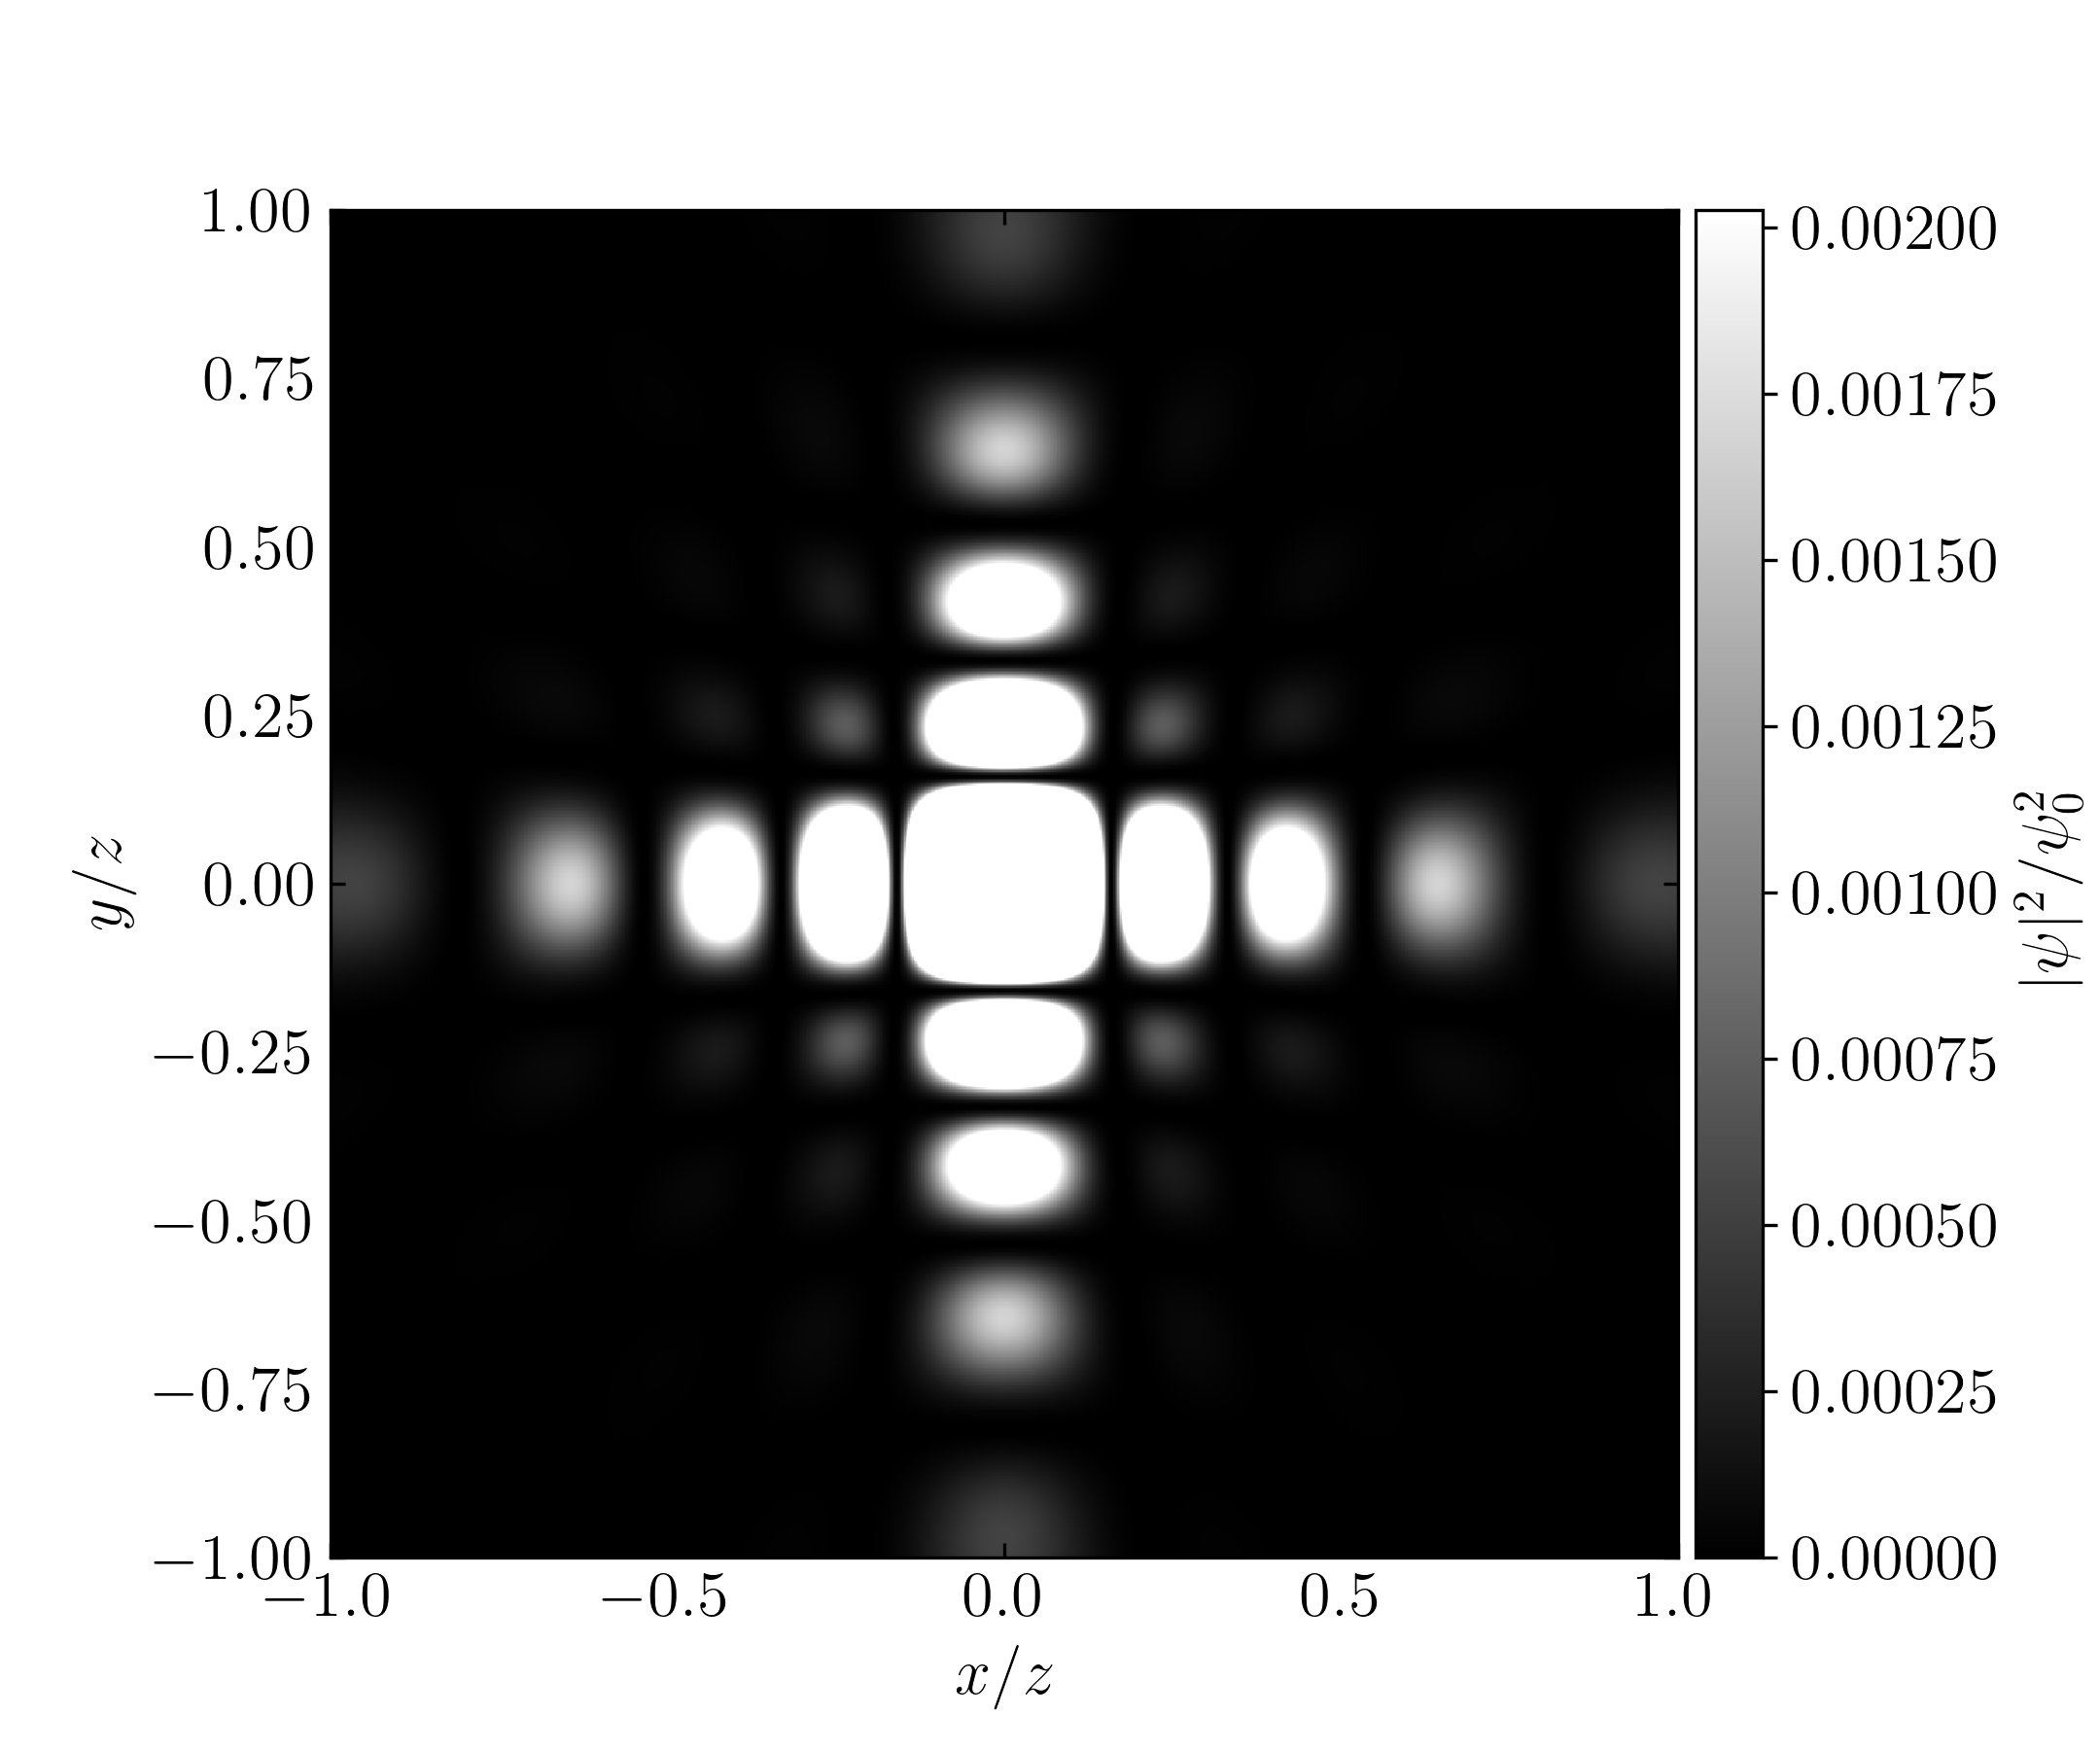
\includegraphics[width=0.8\textwidth]{p2a.png} 
\end{center}
This is the expected Fraunhofer diffraction pattern for a rectangular aperture.

(b) As $b\to0$, $kby/r\to0$ and by L'Hopital's rule,
$\lim_{x\to0}\t{sinc}(x)=\lim_{x\to0}\cos(x)=1$. A plot of $\t{sinc}(x)$ is
provided below, where we can see more clearly the behavior of this function at
small $x$.
\begin{center}
    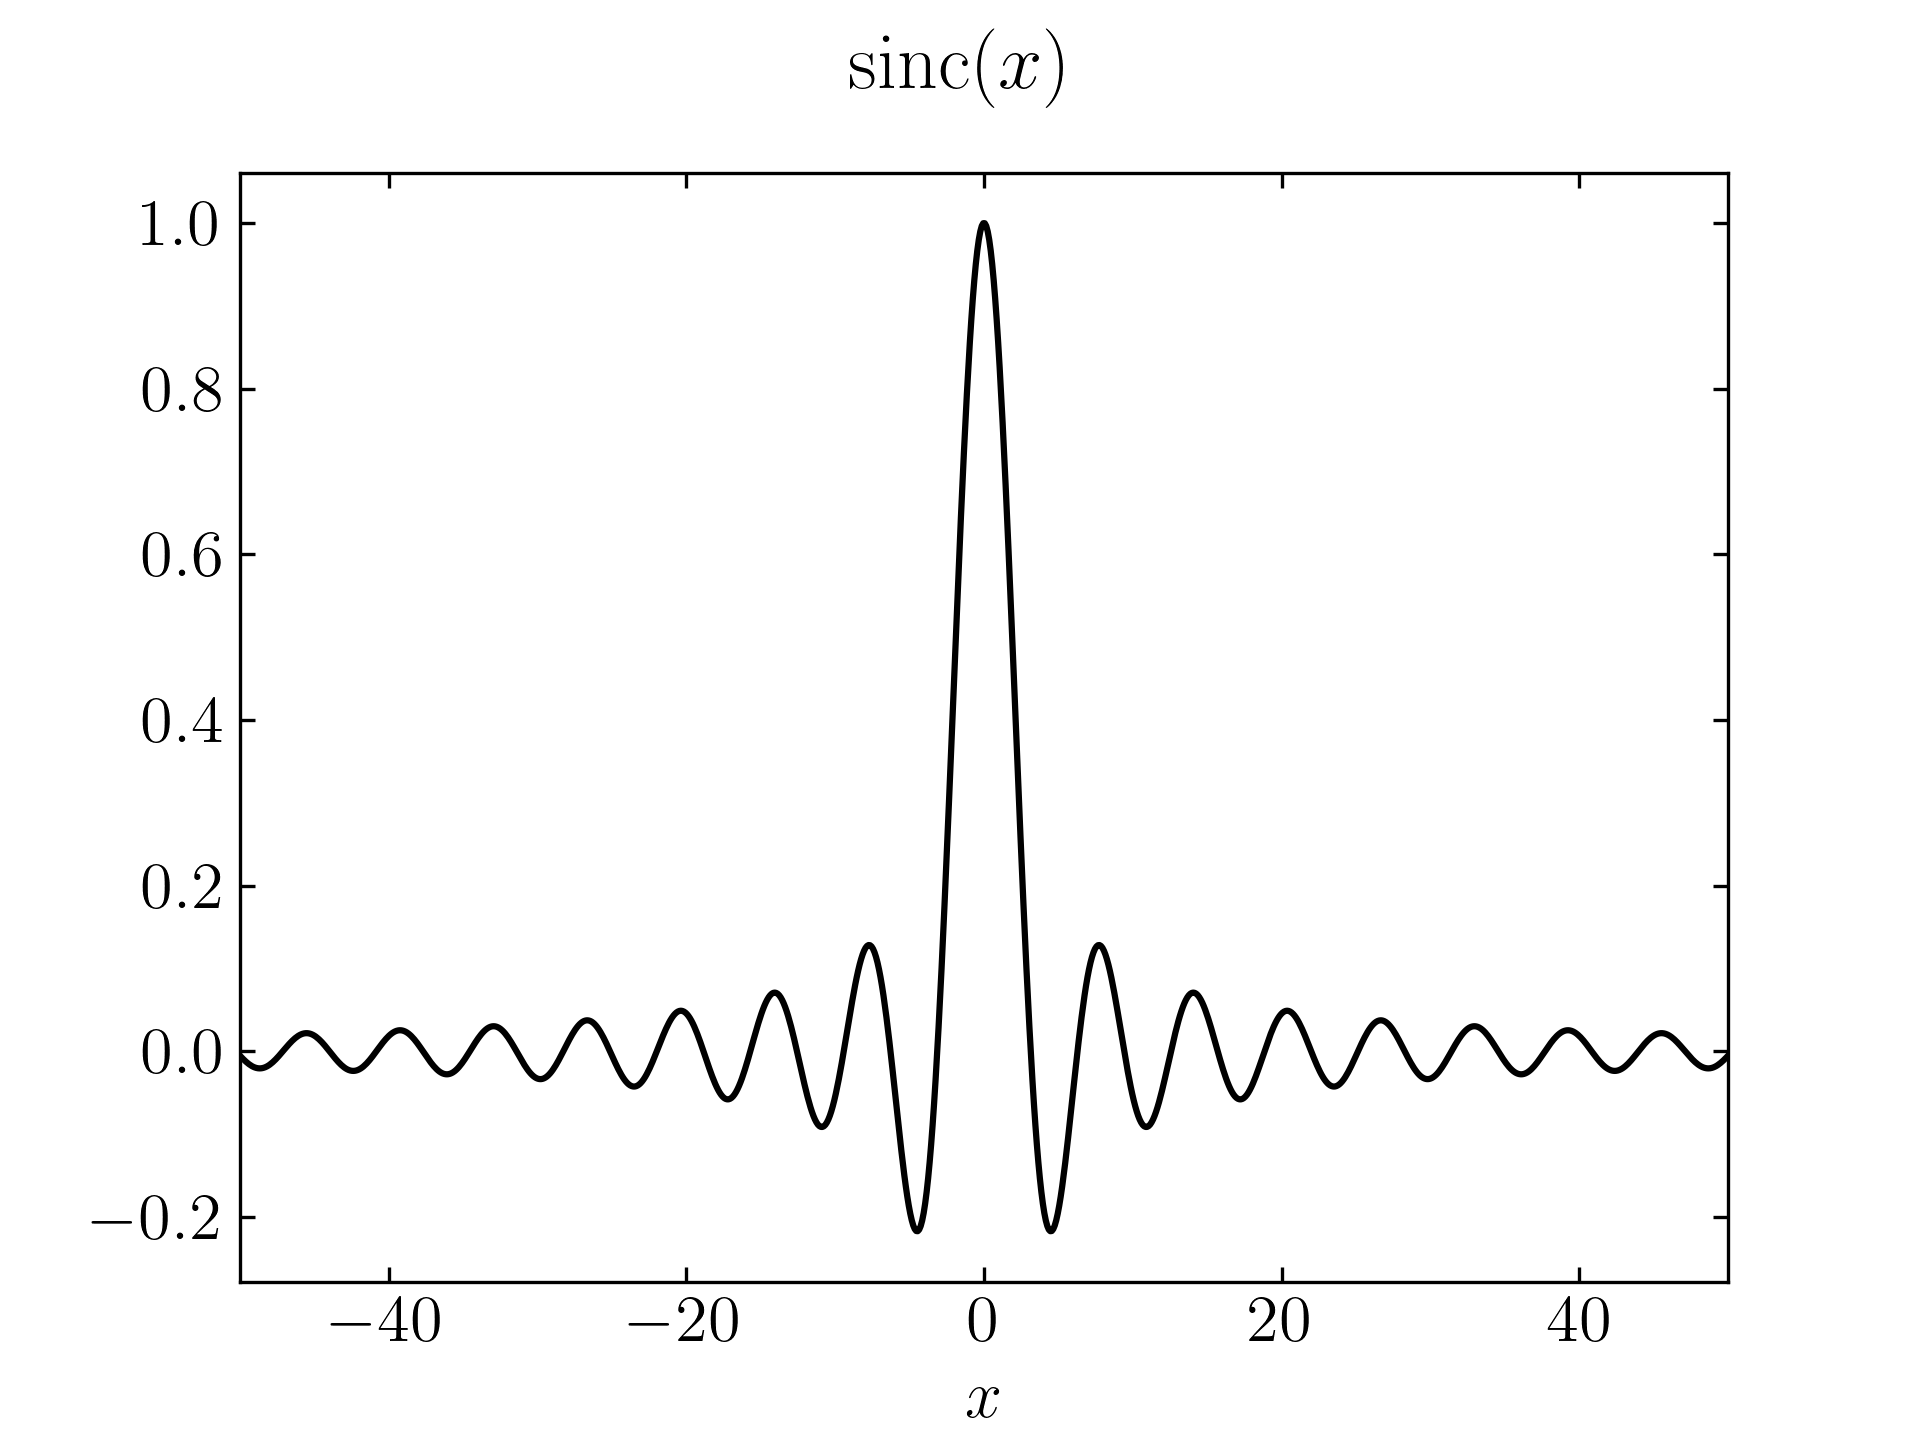
\includegraphics[width=0.6\textwidth]{p2b.png} 
\end{center}

Thus, keeping
$\hat{E}_0=2b\psi_0$ finite, the intensity becomes
\begin{equation}\label{p2b:I}
    \abs{\psi}^2=\frac1{4\pi^2}\frac{(ka)^2}{(kz)^2}k^2\hat{E}_0^2\t{sinc}^2\qty(ka\frac{x}{z}),
\end{equation}
which effectively turns into a 1-dimensional pattern, as the $y$ dependence dies
out due to the limit of $\t{sinc}(kby/r)$. A plot of the intensity \eqref{p2b:I}
is given below, where $z=10a$.
\begin{center}
    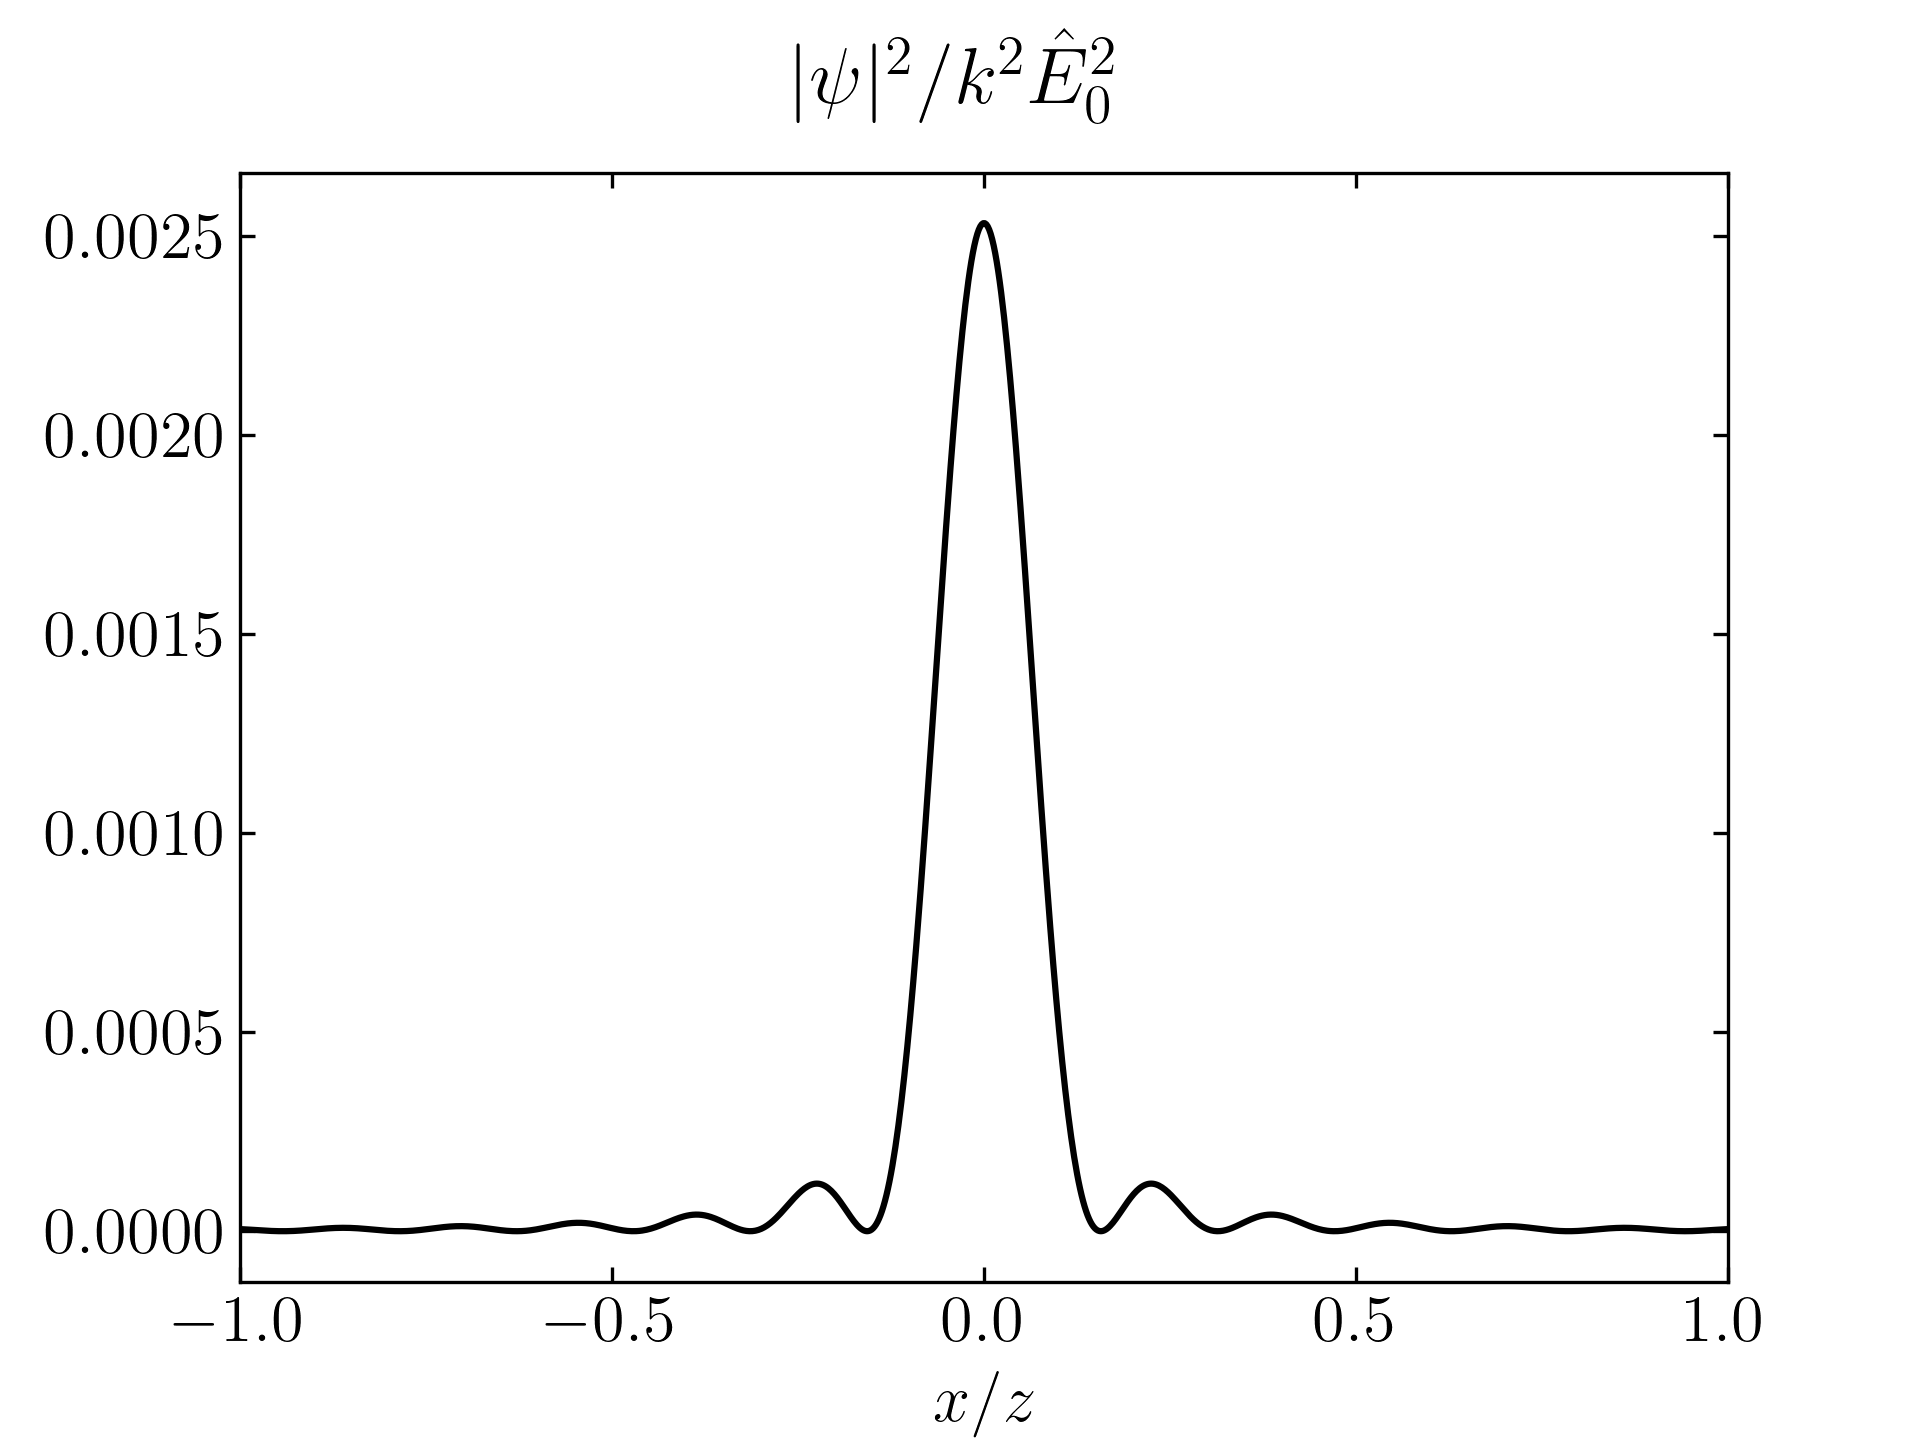
\includegraphics[width=0.8\textwidth]{p2b2.png} 
\end{center}

(c) The form of $\psi$ stays the same, but now we integrate over two openings
$S=S_+\cup S_-$ where $S_\pm=\qty[\pm d-a,\pm d+a]\times[-b,b]$. Again using
(10.108, Jackson), we calculate
\begin{align}
    \psi_\pm
    &=\frac{k}{4\pi i}\frac{e^{ikr}}{r^2}
    \int_{S_\pm}e^{-ik(xx'+yy')/r}\vb{x}\vdot(-\zhat)\psi_0
        e^{-i\omega t}\notag\\
    &=\frac{i\psi_0}{\pi}e^{i(kr-\omega t)}\frac{kz}{r^2}
    \int_{[\pm d-a,\pm d+a]}dx'\int_{-b}^bdy'e^{-ik(xx'+yy')/r}\notag\\
    &=\frac{4i\psi_0}{\pi}e^{i(kr-\omega t)}\frac{z}{kxy}e^{\mp
    ikdx/r}\sin\qty(ka\frac{x}{r})\sin\qty(kb\frac{y}{r}).
\end{align}
Then it follows that
\begin{equation}
    \psi=\psi_++\psi_-
    =\frac{8i\psi_0}{\pi}e^{i(kr-\omega
    t)}\frac{z}{xy}\cos\qty(kd\frac{x}{r})\sin\qty(ka\frac{x}{r})\sin\qty(kb\frac{y}{r}),
\end{equation}
and the intensity is
\begin{align}\label{p2c:I}
    \abs{\psi}^2
    &=\frac{64\psi_0^2}{\pi^2}\frac{z^2}{k^2x^2y^2}\cos^2\qty(kd\frac{x}{r})\sin^2\qty(ka\frac{x}{r})\sin^2\qty(kb\frac{y}{r})\notag\\
    &\approx\frac{16\hat{E}_0^2}{\pi^2}\frac1{x^2}\cos^2\qty(kd\frac{x}{r})\sin^2\qty(ka\frac{x}{r})\t{sinc}^2\qty(kb\frac{y}{z})\tag{$y\ll
    z$}\\
    &\approx\frac{16}{\pi^2}\frac{(ka)^2}{(kz)^2}\cos^2\qty(kd\frac{x}{z})
    \t{sinc}^2\qty(ka\frac{x}{z}),
\end{align}
where we have also assumed $x\ll z$ and $b\to0$. A plot of this intensity is 
given below.
\begin{center}
    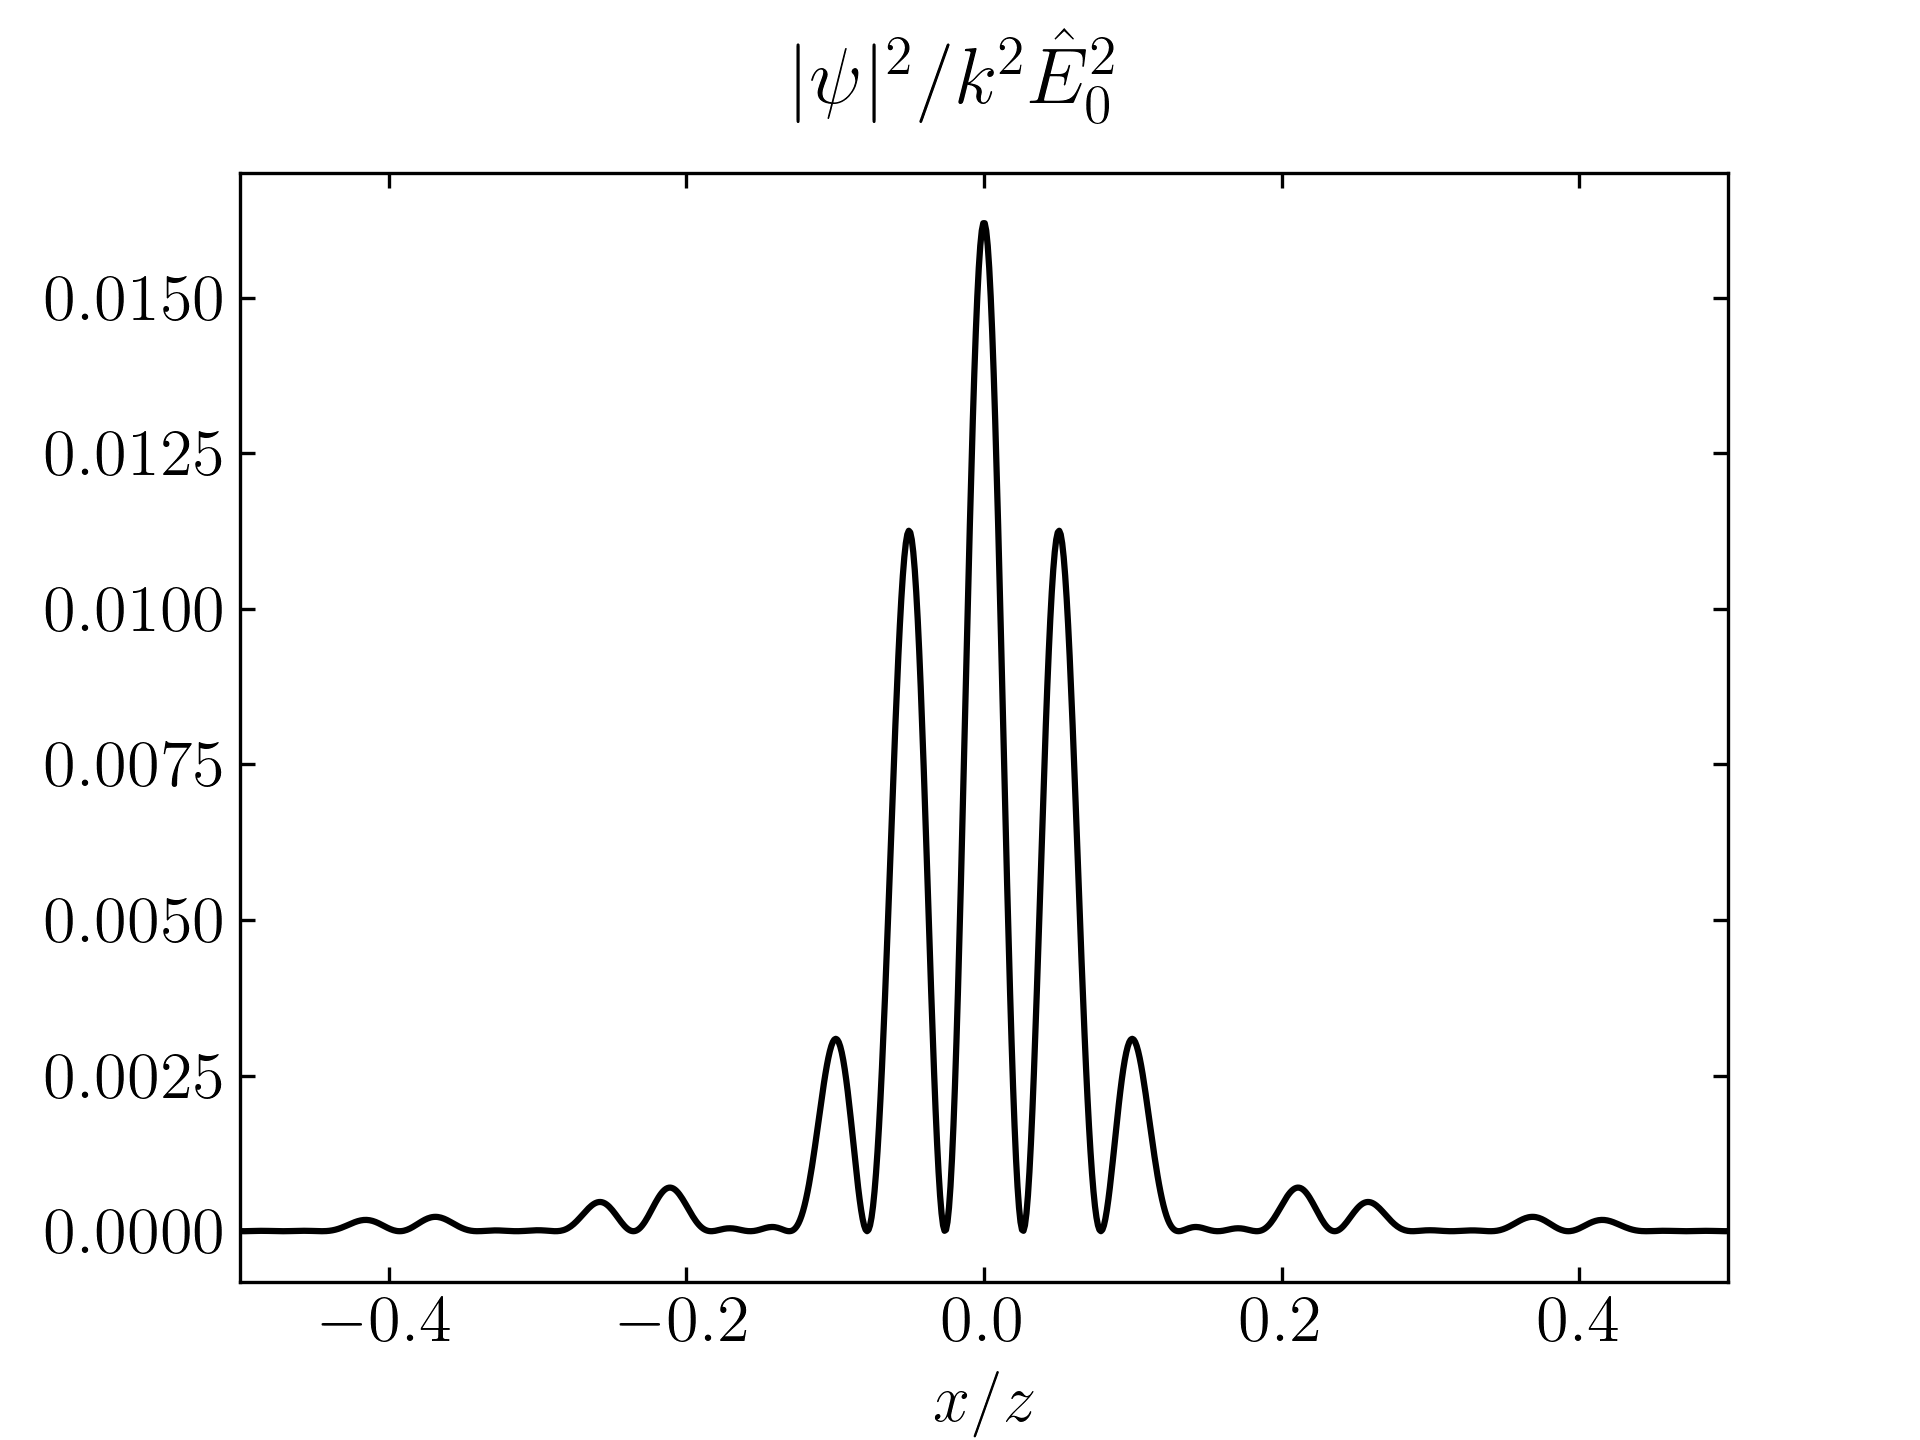
\includegraphics[width=0.8\textwidth]{p2c.png} 
\end{center}
Here we observe clusters of peaks due to interference between the two slits, as
expected.

\end{solution}
\end{problem}
\newpage
%%%%%%%%%%%%%%%%%%%%%%%%%%%%%%%%%%%%%%%%%%%%%%%%%%%%%%%%%%%%%%%%%%%%%%%%%%%%%%%
%%%%%%%%%%%%%%%%%%%%%%%%%%%%%%%%%%%%%%%%%%%%%%%%%%%%%%%%%%%%%%%%%%%%%%%%%%%%%%%
\begin{problem}{M.3}[A moving car]
Consider a car with length $l$, and choose the origin in its rest frame such
that the front of the car is at $x_F=0$, and the rear of the car is at $x_R=l$.

(a) Move to an inertial frame with coordinates $x',t'$ where the car is moving
to the left with constant velocity $v$. Find an equation relating $x_F'$ and
$t_F'$ (the worldline of the front of the car in this frame), and another
equation relating $x_R'$ and $t_R'$ (the world line of the back of the car in
this frame).

(b) Use your results from the previous part to obtain the length of the car in
the primed frame in terms of $l$ (that is, rederive length contraction from your
results). Also, what is the slope of the two worldlines in the spacetime diagram
with $ct'$ the vertical axis and $x'$ the horizontal axis?

(c) The car has a resting length of $l=5$\,\si{m}, a rest mass of 2000\,\si{kg},
and in the primed frame is moving at $3c/5$. Find the energy and momentum of the
car in its rest frame, and the energy, momentum and length of the car in the
moving frame. (The speed of light is $3\times10^8$\,\si{m/s}.)
\begin{solution}
(a) By Lorentz transformation, we can write the transformed (primed) coordinates
as
\begin{equation}
    \mqty(ct_F'\\x_F')=\gamma\mqty(1&-\beta\\-\beta&1)\mqty(ct_F\\x_F)
    =\gamma\mqty(ct_F\\-\beta ct_F),
\end{equation}
where we have set $x_F=0$ in the rest frame, $\beta=vc$ and
$\gamma=1/\sqrt{1-\beta^2}$. Eliminating $ct_F$, we can write $x_F'=-\beta
ct_F'$. Similarly, for the rear of the car,
\begin{equation}
    \mqty(ct_R'\\x_R')=\gamma\mqty(1&-\beta\\-\beta&1)\mqty(ct_R\\x_R)
    =\gamma\mqty(ct_R-\beta l\\-\beta ct_R+l).
\end{equation}
Eliminating $ct_R$, we can write $x_R'=-\beta\qty(\gamma ct_R)+\gamma l
=-\beta ct_R'+l/\gamma$.

(b) In the primed coordinates, the length is measured at the same time
$t_F'=t_R'=t'$. So
\begin{equation}
    l'=x_R'-x_F'=l/\gamma-\beta c(t_R'-t_F')=l/\gamma.
\end{equation}
This is length contraction. From our results in part (a), the slope of both
worldlines is $-1/\beta$. The velocity is negative because it moves to the left.

(c) In the rest frame, the car is not moving by definition, so the momentum is
$p=0$, and the rest energy is $E=mc^2\approx1.12\times10^{30}$\,\si{GeV}. Now,
by Lorentz transformation, the four-momentum in the primed coordinates is
\begin{equation}
    \mqty(E'/c\\p')=\gamma\mqty(1&-\beta\\-\beta&1)\mqty(E/c\\p).
\end{equation}
Thus, the energy is the inertial frame is $E'=\gamma E=\gamma
mc^2=mc^2/\sqrt{1-\beta^2}$. With $\beta=3/5$,
$E'\approx1.4\times10^{30}$\,\si{GeV}. The momentum in the inertial frame is
\begin{equation}
    p'=-\gamma\beta mc=m(-\gamma \beta c)
    \approx-4.5\times10^{11}\,\si{kg m/s}.
\end{equation}
Note that it is negative because the car moves in the negative direction in the
inertial frame. From part (b), the contracted length is $l'=l/\gamma=4$\,\si{m}.
\end{solution}
\end{problem}
\newpage
%%%%%%%%%%%%%%%%%%%%%%%%%%%%%%%%%%%%%%%%%%%%%%%%%%%%%%%%%%%%%%%%%%%%%%%%%%%%%%%
\end{document}
